\documentclass[conference]{IEEEtran-COPS}
% !TEX root =  ../main.tex

% uncomment for submission
%\RenewDocumentCommand\todo{m}{}
%\RenewDocumentCommand\rev{+m}{#1}
%\RenewDocumentCommand\checkNum{+m}{#1}

% only required for the template
\NewDocumentCommand{\cmd}{m}{{\ttfamily\textbackslash{#1}}}


\usepackage{framed}

% Please note: Apart from changing title, keywords, and
% sections, it should not be necessary to edit this file.
% Add your customizations to the preface.tex file.

% Please note: The IEEEtrans-COPS document class only adds
% minor changes on top of the IEEEtrans class. Please open
% the corresponding .cls file to see or adapt the changes.

\begin{document}

\title{Conference Paper Title}

\author{\IEEEauthorblockN{1\textsuperscript{st} Given Name Surname}
\IEEEauthorblockA{\textit{dept. name of organization (of Aff.)} \\
\textit{name of organization (of Aff.)}\\
City, Country \\
email address or ORCID}
\and
\IEEEauthorblockN{2\textsuperscript{nd} Given Name Surname}
\IEEEauthorblockA{\textit{dept. name of organization (of Aff.)} \\
\textit{name of organization (of Aff.)}\\
City, Country \\
email address or ORCID}
\and
\IEEEauthorblockN{3\textsuperscript{rd} Given Name Surname}
\IEEEauthorblockA{\textit{dept. name of organization (of Aff.)} \\
\textit{name of organization (of Aff.)}\\
City, Country \\
email address or ORCID}
}

\maketitle
\maketitle

\begin{abstract}
% !TEX root =  ../main.tex
Lorem ipsum dolor sit amet, consectetur adipiscing elit, sed do eiusmod tempor incididunt ut labore et dolore magna aliqua. Ut enim ad minim veniam, quis nostrud exercitation ullamco laboris nisi ut aliquip ex ea commodo consequat. Duis aute irure dolor in reprehenderit in voluptate velit esse cillum dolore eu fugiat nulla pariatur. Excepteur sint occaecat cupidatat non proident, sunt in culpa qui officia deserunt mollit anim id.
\end{abstract}

\begin{IEEEkeywords}
component, formatting, style, styling, insert
\end{IEEEkeywords}

% !TEX root =  ../main.tex
\section{Introduction}
\label{sec:intro}

This document is a template for how to write LaTeX documents in the COPS lab for IEEE venues.
This document introduces the \code{IEEEtran-COPS} document class, which extends the base \code{IEEEtran} document class%
\footnote{\url{https://www.ieee.org/conferences/publishing/templates.html} (Oct 2019)}
with some useful additions that we have been frequently using in our lab throughout the years.
The changes are very small and incremental, please check the \code{IEEEtran-COPS.cls} file to inspect the minor differences.

This document also serves as a primer for students that are not too familiar with writing Latex documents yet.
It contains many examples of basic Latex usage that illustrate best practices for how to write good Latex.

% !TEX root =  ../main.tex
\section{Semantic Formatting}

I always compare writing Latex documents to writing HTML websites: You are basically writing content and somehow need to format it to make it readable.
While it is \emph{possible} to use formatting \emph{inline}, like making text {\bf bold} or {\it italic}, this is \emph{highly discouraged} for two reasons:

\begin{enumerate}
%
\item Your paper will evolve over time and you will change the details of your formatting throughout this journey.
Let's assume that you want to highlight code fragments or file names consistently and you start by simply using italics for that, like {\it myfile.txt}.
At some point, you want to change that to small capitals, so you have to go through the whole paper and manually all usages to, for example, {\sc myfile.txt}.
This is a a) lot of effort and b) very error prone.
%
\item It is more than likely that your paper will be rejected and that you have to resubmit it somewhere else (sorry for breaking the news ;)).
As different venues often follow different templates, a \emph{reformat} is often necessary.
%
\end{enumerate}

A much better alternative to inline formatting is to use semantic \emph{macros} like \cmd{emph} ("emphasize"), which templates often redefine to match their style.
These macros serve a similar role for Latex than CSS would for HTML.
Instead of worrying about the concrete formatting, you use them to express that you want to highlight somethings or you express a specific concept, like a \cmd{section}, a \cmd{paragraph}, or a list \cmd{item}.
The formatting of these macros is then done centrally.

The template comes with the predefined macros \cmd{code} (that we use to highlight inline source code or paths like \code{MyClass.class}) and \cmd{tool} (that we use to highlight tool names, like \tool{Java} or \tool{Maven}).
First of all, using these macros will improve the readability of your document and using semantic macros makes it very easy to change formatting in a central place.
Defining a macro is not that hard, but there are two styles: \emph{commands} and \emph{environments}.

\paragraph{Commands}

\NewDocumentCommand{\withparams}{mm}{You can just use parameters by referring to their number, like #1 or #2}
\NewDocumentCommand{\optparams}{mO{XY}}{m:#1, opt:#2}
\NewDocumentCommand{\noparams}{}{No parameters}

New commands can be easily defined in Latex with the \cmd{NewDocumentCommand} command, check the source code of this section for examples.
A command can have parameters (\withparams{a}{b}), optional parameters (\optparams{c}), but it does not have to (\noparams{}).
Once defined, the command is available to all \emph{following} Latex source, so it is recommended to define your commands in the \code{preface.tex} file.


\paragraph{Environments}

As an alternative, you can define environments.
Their definition is similar to commands (e.g., they also support parameters), but the key idea is to define the \emph{before} part and the \emph{after} part of your content.
For example, we can define a \code{results} environment that adds information before and after your content and adds a box around it (Using the \code{framed} package that is imported in the \code{preface.tex}).

\NewDocumentEnvironment{resultBox}{mm}%
% before:
{\begin{framed} \noindent #1}
% after:
{#2 \end{framed}}

This definition can then be used to create a results box:

\begin{resultBox}{AAA}{BBB}
Some results ...
\end{resultBox}

The benefit of using this custom environment over directly using a \code{framed} environment everywhere is clear.
Additional information can be trivially add, like a findings counter, or a reformat of the box design is a central change.

\paragraph{Please note} You are not going to master commands and environments over night (and you do not have to), but it is good to understand how to use them as they can make your documents more maintainable and you life so much easier.

% !TEX root =  ../main.tex
\section{Structuring the Document}

Latex has a plethora of different methods to structure a document.
Pick the right methods depending on the situation and the amount of content to structure, not one methods is always preferable.
This section is filled with a lot of generated text to illustrate how the resulting structure looks like.

\subsection{Structuring with Subsections}

Latex has multiple strucutral elements, like \cmd{section}, \cmd{subsection} et cetera.
These elements are \emph{visually} very heavy and represent a large break for the reader.
Do not over-use them.

\subsubsection{First Subsection}
Lorem ipsum dolor sit amet, consectetur adipiscing elit, sed do eiusmod tempor incididunt ut labore et dolore magna aliqua. Ut enim ad minim veniam, quis nostrud exercitation ullamco laboris nisi ut aliquip ex ea commodo consequat.

\subsubsection{Another Subsection}
Lorem ipsum dolor sit amet, consectetur adipiscing elit, sed do eiusmod tempor incididunt ut labore et dolore magna aliqua. Ut enim ad minim veniam, quis nostrud exercitation ullamco laboris nisi ut aliquip ex ea commodo consequat.

\subsubsection{Last Subsection}
Lorem ipsum dolor sit amet, consectetur adipiscing elit, sed do eiusmod tempor incididunt ut labore et dolore magna aliqua. Ut enim ad minim veniam, quis nostrud exercitation ullamco laboris nisi ut aliquip ex ea commodo consequat.

\subsection{Structuring with Named Paragraphs}

In addition to \emph{regular} paragraphs, Latexsupports \emph{named} paragraph with a short title through the \cmd{paragraph} command.

\paragraph{First Paragraph} Lorem ipsum dolor sit amet, consectetur adipiscing elit, sed do eiusmod tempor incididunt ut labore et dolore magna aliqua. Ut enim ad minim veniam, quis nostrud exercitation ullamco laboris nisi ut aliquip ex ea commodo.

Lorem ipsum dolor sit amet, consectetur adipiscing elit, sed do eiusmod tempor incididunt ut labore et dolore magna aliqua. Ut enim ad minim veniam, quis nostrud exercitation ullamco laboris nisi ut aliquip ex ea commodo.

\paragraph{Another One} Lorem ipsum dolor sit amet, consectetur adipiscing elit, sed do eiusmod tempor incididunt ut labore et dolore magna aliqua. Ut enim ad minim veniam, quis nostrud exercitation ullamco laboris nisi ut aliquip ex ea commodo.

\paragraph{The last Paragraph} Lorem ipsum dolor sit amet, consectetur adipiscing elit, sed do eiusmod tempor incididunt ut labore et dolore magna aliqua. Ut enim ad minim veniam, quis nostrud exercitation ullamco laboris nisi ut aliquip ex ea commodo.


\subsection{Structuring with Description Lists}

Description lists are, well, lists, so they should be wrapped in text and not stand alone.

\begin{description}
%
\item[Foo] Lorem ipsum dolor sit amet, consectetur adipiscing elit, sed do eiusmod tempor incididunt ut labore et dolore magna aliqua. Ut enim ad minim veniam, quis nostrud exercitation ullamco laboris nisi ut aliquip ex ea commodo consequat.
%
\item[Bar] Lorem ipsum dolor sit amet, consectetur adipiscing elit, sed do eiusmod tempor incididunt ut labore et dolore magna aliqua. Ut enim ad minim veniam, quis nostrud exercitation ullamco laboris nisi ut aliquip ex ea commodo consequat.
%
\item[Baz] Lorem ipsum dolor sit amet, consectetur adipiscing elit, sed do eiusmod tempor incididunt ut labore et dolore magna aliqua. Ut enim ad minim veniam, quis nostrud exercitation ullamco laboris nisi ut aliquip ex ea commodo consequat.
%
\end{description}

Description lists should also not end a section.
At the very least, you should write a summary of the contents.
If the description list is the only content of a section though, you should really think about whether it is the right choice.


\subsection{Basic Paragraphs and Whitespace}

Structure helps to read a document, however, too much structure interrupts the flow.
Sometimes it is easier to use simple paragraphs and whitespace to improve readbility.

A simple paragraph already signals to the reader a break in the argumentation or a shift in direction.
The direction should not fundamentally change though, consider a paragraph a simple breather that help the reader to understand when to stop and think about the current argument.

\medskip
Larger breaks in the argumentation can be indicated with a \cmd{smallskip} or a \cmd{medskip}.
I would recommend to pick what looks better for your paper or how desperate you are for space.
Most importantly, do not jump between \cmd{smallskip} and \cmd{medskip}, but use one command consistently.

% !TEX root =  ../main.tex
\section{Citations \& References}

Citing papers or external resources is very easy in Latex.
In our field, the convention is to use the first authors \emph{last name} and \emph{et al.} to indicate that there were more authors. For example: Smith et al.~\cite{AAI34-icse} were the first to introduce foobar by perfoming blah, which lead to blubb.
Please note the {\textasciitilde} in the Latex code, which makes sure that the citation number will never break into the next line alone, which would look weird.
This style of citation also works for all other venues like journals~\cite{DE23-emse} or books~\cite{ABC12-abc}.
It is also possible to cite websites~\cite{Pue08}, however, these pages should then contain relevant content for the paper.
When the reference is only linking to a tool, it is often better to use a footnote for that.%
\footnote{\url{https://www.maven.org}, accessed: 10-Nov-2023}

As an important note, make sure that you \emph{never} use a citation as an object in a sentence (like "As shown in~\cite{DE23-emse}, ..."), this is very bad style.
Instead, either name the authors (e.g., "Foo et al.~\cite{DE23-emse} have shown ...") or formulate it as a general statement (e.g., "Prior research has shown that ... \cite{DE23-emse}").

\medskip
Within a document, it is possible to refer to each element that has a counter, like sections or figures.
When a \cmd{label} has been added to these elements, one can use \cmd{ref} to refer back to them.
This way, it is possible to refer back to Section~\ref{sec:intro} or Figure~\ref{fig:abstract-image}.
Please note that both Section and Figure are uppercase and that the Latex code again uses a {\textasciitilde} to prevent unfortunate linebreaks.
Please also not that the prefixes \code{fig:} and \code{sec:} have been added \emph{by convention} to the \cmd{label} and \cmd{ref}.

To make it easier to reference elements in the document, the template supports the \code{cleverref} package.
It is possible to just use \cmd{Cref} to refer to the elements, without explicitly typing the elements name.
For example, note in the Latex source how the following reference to \Cref{fig:abstract-image} does not contain the "Figure", which appears in the .pdf though.


% !TEX root =  ../main.tex
\section{Images}

\begin{figure}
\centering
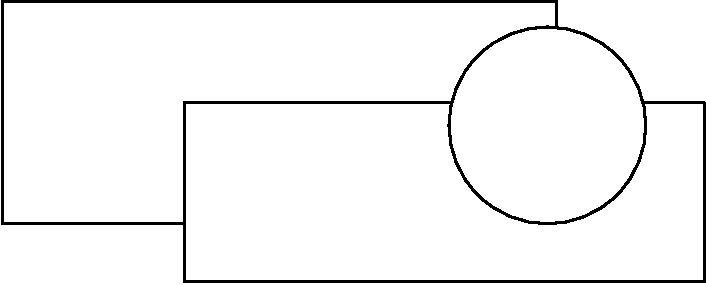
\includegraphics[width=0.8\columnwidth]{images/abstract-image}
\caption{This is an abstract image}
\label{fig:abstract-image}
\end{figure}


You can see an abstract image in Figure~\ref{fig:abstract-image}.
% !TEX root =  ../main.tex
\section{Tables}

\begin{table}
\centering
\caption{This is a basic table}
\label{tab:basic}
\begin{tabular}{@{}lllr@{}}
\toprule
\multicolumn{2}{c}{\bf Name} & \\
\cmidrule{1-2}
First & Last & {\bf Nationality} & {\bf Number} \\
\midrule
John  & Doe & US & 123.0 \\
Max & Mustermann & Germany & 1.7 \\
\bottomrule
\end{tabular}
\end{table}

This section shows a basic example in Table~\ref{tab:basic}.
Creating nice looking tables in Latex is not difficult when basic rules are being followed.
I warmly recommend to study the article \emph{"Small Guide to Making Nice Tables"}~\cite{Pue08}, which give a very useful primer.

The most complex part of Latex tables is the \code{tabular} environment, because it can become very complex very fast.
As such, I recommend to treat it like a picture and just move it out of the main document.
% !TEX root =  ../main.tex
\section{Writing Process}

Writing is a very iterative process and over time the written text gets \emph{massaged} into its final form.
To make this process easy, it is recommended to keep as much information as possible in the document and not use external documents for planning, communication, or extra notes.

The paper will be very messy initially, but the paper should make it trivial to get an estimate of the current state \emph{on a quick glance}.
As such, we will use various Latex macros to "label" the text.

The most basic indicator is \cmd{todo}.
Use it to note down ideas during a discussion or when you do not have the time to elaborate something.
\todo{Extend this explanation}

Once you had time to add more information, the text is likely still in a rough shape.
Use \cmd{rev} to mark text that is \emph{in principal} already \emph{content complete}, but that still requires a thorough revision.
\rev{This makes it a lot easier to collaborators to understand which parts are still rough or which parts should be considered "done".

Do not be shy and remove the \cmd{rev} tag as soon as you think that the text is polished.
Should a collaborator feel that more work is need in a section, they will add the marker back.}

Scientific paper usually contains many numbers.
To make it easy to spot the numbers when you check your paper for consistency before submission, wrap them in a \cmd{checkNum} command.
You will find it easier to spot the \checkNum{five} mentions of the \cmd{cmd} command in your paper when the number is highlighted.

All these commands are predefined in the COPS-flavored document class that extends the basic IEEE template.
You want to make sure that the formatting is removed before you submit the paper.
You can find commented out \cmd{RenewCommand} instructions in the \code{preface.tex}, once you uncomment them, all formatting and extra text is gone.
Try it out!

Finally, do not include questions or instructions as comments, as someone who will only read the PDF won't see them.
Also, trust your version control system and avoid keeping commented text in your paper.


% !TEX root =  ../main.tex
\section*{Acknowledgment}

The acknowledgments usually refer to the funding agencies that have supported the work and to collaborators that have added substantial contributions to the paper.
This section is usually not included for the review version of the paper, as it easily exposes the identity of the researchers.



\balance
\bibliographystyle{IEEEtran}
\bibliography{references}

\end{document}
